\chapter{Introduction}
The use of video-based surveillance system has permeated the society as a core technology for security and consumer applications. Over the past decade, both the private and public sectors have benefited from the ease of implementation along with the low implementation cost.
Retail stores, shopping malls, public places, and private homes have equipped themselves with closed-circuit television (CCTV) systems as a means for security. Figure \ref{fig:examplescenes} shows the use of video surveillance system in the various described scenes.
Furthermore, with the rise of Internet of Things (IoT), Big Data and even the
Fourth Industrial Revolution (Industry 4.0) over the recent years, there has been a deeper thirst among researchers to find practical use cases by bridging %existing
data with technology to bring about a new wave of research.

\begin{figure}[!htb]
 \centering
 \resizebox{\textwidth}{!}{
 \begin{tabular}{ccc}
 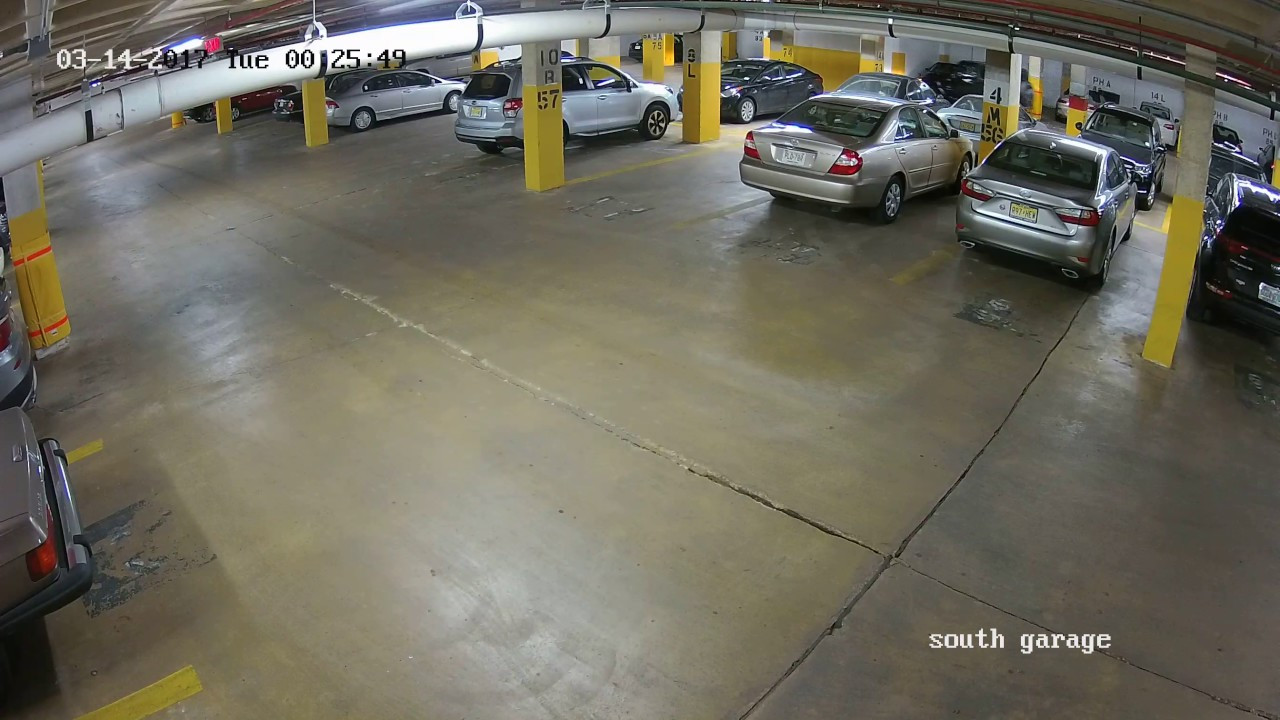
\includegraphics[width=0.4\linewidth]{image/screenshots/carparkindoor.jpg} &
 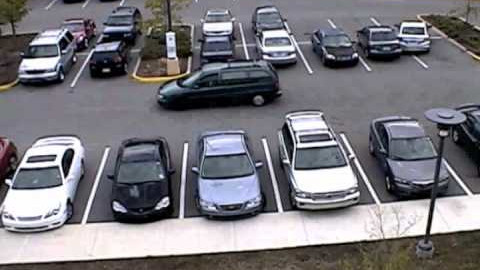
\includegraphics[width=0.4\linewidth]{image/screenshots/carparkoutdoor.jpg} &
 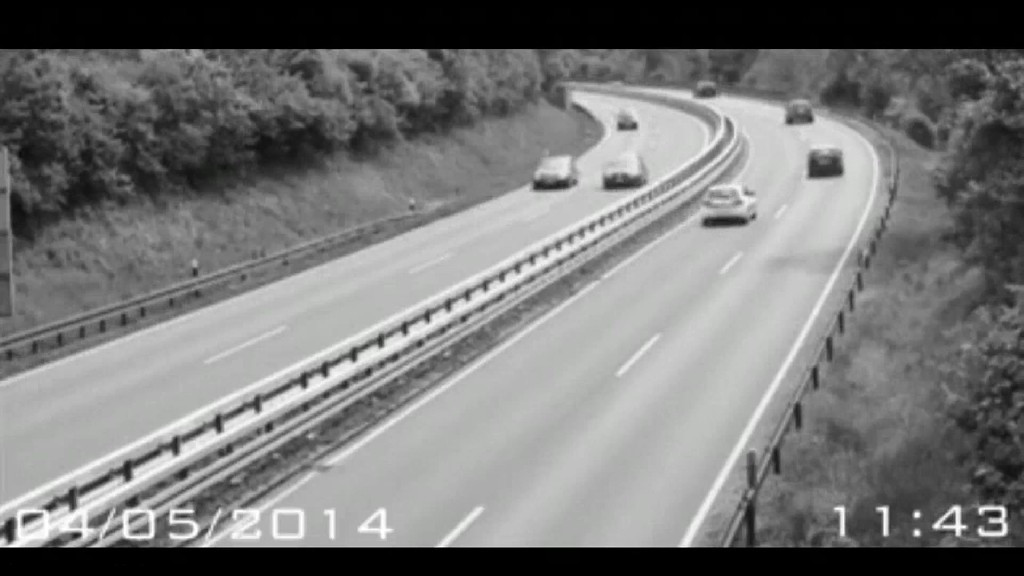
\includegraphics[width=0.4\linewidth]{image/screenshots/highway.jpg}\\
 (a) Indoor Car Park & (b) Outdoor Car Park & (c) Highway\\
 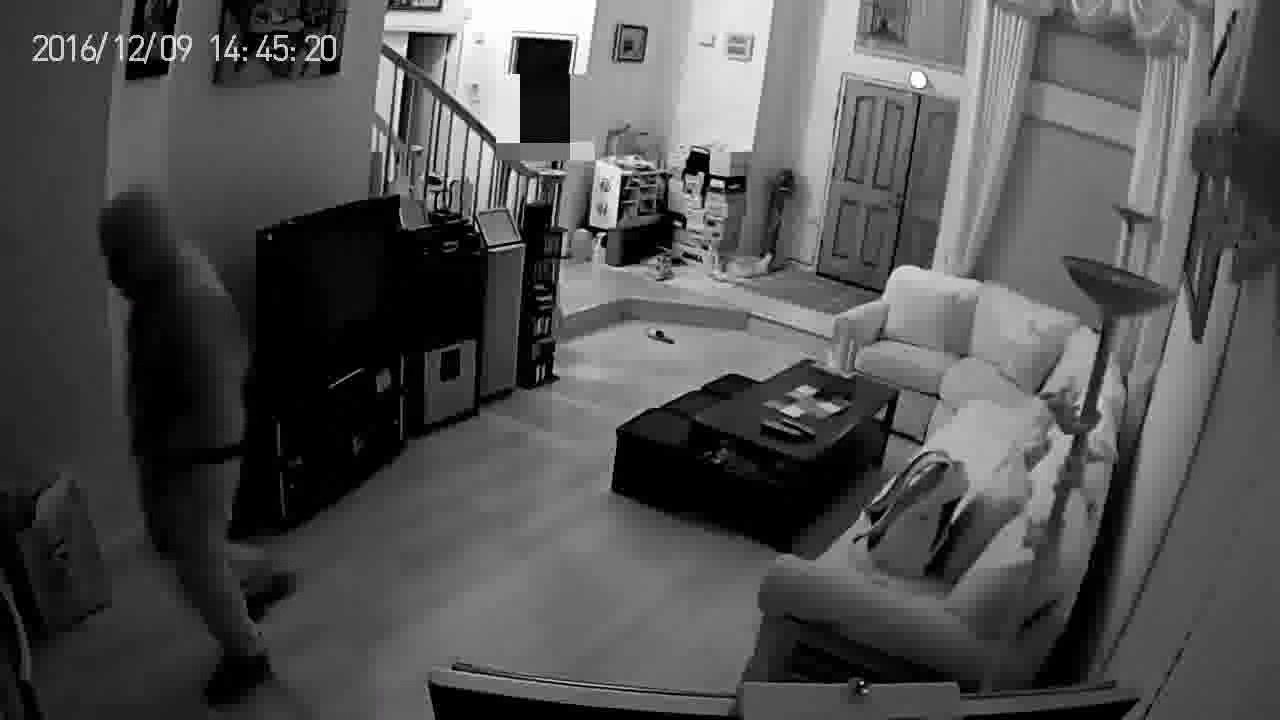
\includegraphics[width=0.4\linewidth]{image/screenshots/home.jpg} &
 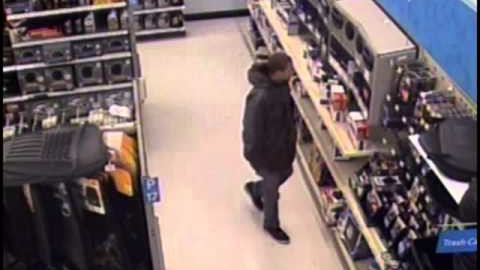
\includegraphics[width=0.4\linewidth]{image/screenshots/retail.jpg} &
 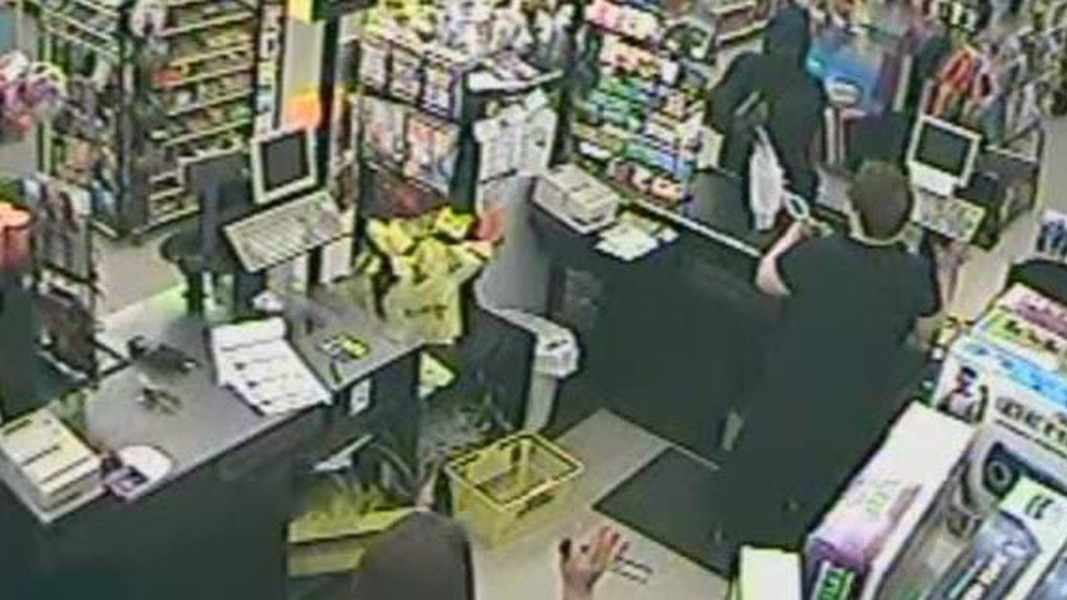
\includegraphics[width=0.4\linewidth]{image/screenshots/robbery.jpg}\\
 (d) Home & (e) Retail & (f) Retail (Robbery) \\
 \end{tabular}}
\caption{Example of Surveillance using Video Data in Various Scenes}
\label{fig:examplescenes}
\end{figure}

\section{Research Overview}
\label{section:introduction}

The growth of the surveillance industry has also brought forth the rise of
constant streams of video data. According to a research done by the IHS Markit
(a leading source of information, insights, and analytics), the average data
generated daily by new surveillance camera shipped globally would have grown up to 2,500 Petabytes daily by 2019~\cite{woodhouse2016big}. 
A study by Seagate Techology LLC suggested that approximately 566 petabytes of data was generated in a single day from new video surveillance cameras installed worldwide in 2016. Furthermore, this number would continue grow and reach an estimated 3,500 Petabytes by 2023~\cite{mrfr_2021}.
Within the span of several minutes, hundreds of thousands %if not
to millions of hours worth of video data are filling up database warehouses across the globe.
%by the second.
While these video footages are useful when it is needed (for example, when
dealing with crime scene investigations), in most situations, these data are stored and left unprocessed, taking up additional storage space which further compounds its overhead cost.
This reactive-approach towards surveillance systems makes it slow and difficult for investigators to manually inspect the playback of these crime scene clips one at a time.

Looking from the entertainment sector, multimedia contents are dished out at a
remarkable rate. These digital contents are being pushed into data warehouses
and consumed by the users on a daily basis. The general public as a whole has
also benefited from the rise of various video search engines and tools such as
Google, YouTube, Dailymotion, and Bing. However, it is unlikely for these
existing technologies to be directly applied towards surveillance video footage
or to excel in finding the desired footages as these video search engines takes
in keyword-based queries which are not domain specific.
% Clearly, the idea of using search engines to retrieve video footage is nothing new. Hence, inspirations are drawn from these technologies and applied to the research problem at hand. %which will be discussed in this work.

\begin{figure}[!hbt]\centering
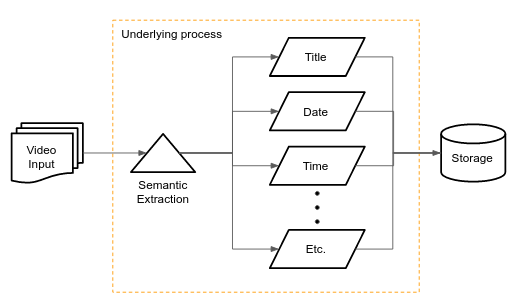
\includegraphics[width=0.9\textwidth]{image/general/simpleframe3.png}
\caption{Generic Semantics Extraction Process}
\label{fig:exampleframework2}
\end{figure}

All of the aforementioned retrieval engine technologies are similar
%have one thing in common, which is
in their underlying process (See Figure \ref{fig:exampleframework2}). First, the process begins with the extraction of video metadata such as title, description, filename, dates, subtitles and various other details that could assist in identifying these footage(s). Next, these videos are typically stored in a database (either entirely or in manually defined segments) along with its corresponding extracted metadata which can be used during the retrieval process. Finally, a text-based query is usually issued, thus resulting in video shots being retrieved and sorted in a way that best
%represents
reflects the similarity to
the query inputted by the end-users.

It is essential now to highlight some inadequacies in this generic process.
Firstly, this process flow cannot be directly applied to generic surveillance video footage as the metadata such as title, description or even tags may not exist in many cases.
For example, a query such as `Select all vehicles entering from Entrance A and turning into Junction B' is difficult for these search engines as it requires domain-specific knowledge for each of these keywords.

Secondly, from the surveillance video footage standpoint, the traditional approach of finding a particular video from a huge collection is typically performed manually. This process would involved an inquirer/user who is required to search for a particular segment of a long spanning footage. Without the help of automatic event extraction procedures or some form of video-based semantics, this may be a tedious process for the user.
%and one or more person-in-charge who manages the video collection.
Drilling further down to the scope of this research, which is based on a car park surveillance setting, the inquirer would typically need to provide vehicle-specific \textit{semantics} such as the time, date, colour of the vehicle, vehicle registration number, and location-in-scene for which an incident had occurred. This necessitates a more contextualised methodology. %In this work, these information are examples of what would be referred to as semantics.

Thirdly, the typical process is likely not efficiently scaled. The end user would have to sift through hours and hours of video data to locate potential video segments that matches the queried information. This %\textit{'reactive-approach'}
process is undeniably time-consuming and laborious, especially when the data in-store grows potentially to a few orders of magnitude larger. While the task is potentially straightforward when there is only one intended video shot with clear-cut definitive time and date given; this process takes enormous effort when details such as the time and date is not given, or even in cases when all the video shots with similar properties are desired within a given time range. Evidently, there exist a gap that can be addressed
%using a \textit{proactive} approach
via a well designed semantic extraction strategy and new query and retrieval techniques which this thesis attempts to address. Figure \ref{fig:observerdatacenter} shows an example of a surveillance control centre where security personnel keep an eye on various scenes.

\begin{figure}[!hbt]\centering
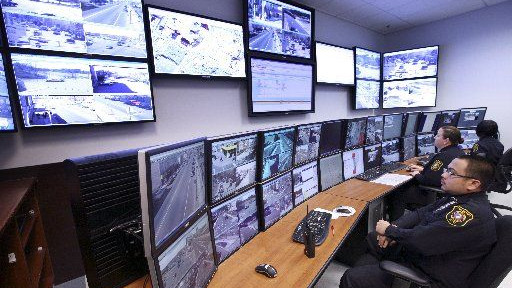
\includegraphics[width=0.8\textwidth]{image/screenshots/observer.jpg}
\caption[Example of Surveillance Control Centre.]{Example of Surveillance Control Centre.
Image reproduced from \citeA{service_2010}.}
\label{fig:observerdatacenter}
\end{figure}

\section{Motivation, Problem Statements and Research Questions}

As described in the previous section, the traditional method used to retrieve desired surveillance video footage is not an effective use of time and manpower. In this section, the motivation to address the topic at hand is further discussed from the computer vision viewpoint.% and natural viewpoint.

%explain what constitutes a good semantic extraction tool and a retrieval engine
%\subsection{Motivation}

%At the frightening collection rate of surveillance video data
In large systems with immense amounts of surveillance data, employing human labour to manually extract information from the video data source will undoubtedly be time-consuming and is extremely labour intensive.
While not impossible, the simple act of watching the same scene over and over again from the video source will put mental and physical strain on the task personnel. When considering as well the amount of video data that has been collected in the past, it may be a cognitively complex task to manually gather insights over time. Thus, providing feasible analyses on the data is extremely difficult without automation.

With the aforementioned disadvantages of performing these tasks traditionally, computer vision techniques can be employed to extract information from video data which can potentially automate many of these processes. As a matter of fact, the use of such techniques is not new. %a generic Computer Vision task is visualised in Figure \ref{fig:genericCV}.
Literature relating to the extraction of vehicle-specific attributes can be found from about two decades ago and it is still an ongoing research area today. Viewing more generally, a bulk of these vehicle-based surveillance research placed their focus on \textit{highway} \cite{yu2017improved, cao2016vehicle, arya2016real, liu2016highway, al2016adaptive}, and  \textit{intersection} \cite{meng2017traffic, choong2017modeling, ren2018learning} scenarios. Among the few rare works \cite{shi2017study, marmol2016quickspot, ling2017identifying} that focus on \emph{car park} scenarios, their primary objective tends to revolve only around identifying the availability of parking spots. Such tasks are independent of the time of occurrence, and execution can be done at any given time according to user needs. Currently, to the best of our knowledge, there has been very little existing works that cater specifically towards the task of retrieving video shots from a long running car park scenario.

The ability to retrieve video shots from such scenario would be useful as it might be able to assist investigators in their quest of finding for a particular event. Similarly, researchers who may be interested in learning how vehicles interact and behave with each other in a car park scenario could also make use of the video shots retrieved. Furthermore, the distribution of vehicle colour from different car parks may suggest preferences of consumers from different regions. Such data would be beneficial to vehicle manufacturers when organising targeted marketing campaigns.

%\begin{figure}[!hbt]\centering
%
\includegraphics[width=.8\textwidth]{image/general/simpleframe.png}
%\caption{Generic Computer Vision Task}
%\label{fig:genericCV}
%\end{figure}

The rise of technology has benefited researchers in the computer vision area greatly due to higher computational power at lower costs. The ability to churn out interpretable and meaningful semantics from raw video footage in a rapid manner has great commercial potential. Even so, there are still plenty of challenges and opportunities which are yet to be solved to improve on existing techniques. As mentioned in Section \ref{section:introduction}, existing popular video retrieval engines such as YouTube generally rely on keyword-based queries. Queries such as 'Selecting all vehicles entering from Entrance (A) and turning into Junction (B)' are less effective as it may require additional labelling or rule creation while it also does not capture the semantic content required by the end-user.

Several authors attempted to solve this challenge,
albeit for generic scenarios,
by proposing the use of example-based queries \cite{zhang2017car, liu2016large, castanon2016retrieval} to facilitate the retrieval process.
These queries typically require end-users to provide inputs in the form of an image or sample of the desired output. While it is possible to provide a thumbnail query image for different scenes (e.g., beach, mountain, waterfall) and objects (e.g., bicycle, pen, lipstick), this is difficult with surveillance video footages as instances are often similar in appearance throughout the recorded duration. Additionally, it would be highly unlikely for end-users to have a copy of the sample footage in order to perform matching against all recorded events.
To tackle this research problem, the following are some research questions which will be addressed in this thesis:
\begin{enumerate}
\item What feasible concepts from existing techniques can we glean and exploit for the purpose of solving the problem?
\item How can we best represent surveillance video footage in the form of higher level semantics? Can vehicle colour and trajectories sufficiently represent events in a car park? 
\item How can we develop retrieval techniques that take in intuitive, flexible and user-friendly query inputs while providing accurate search results that are ranked according to their relevancy to query?
\end{enumerate}


\vspace{1em}
\subsection{Research Objectives}
The objectives of this thesis can be divided into two main interdependent parts. As a whole, the entire work aims to adopt and leverage on existing frameworks to design a feasible object-level \textbf{semantic attributes extraction} and \textbf{retrieval} techniques for \textbf{car park videos}.
With the goal of answering the aforementioned research questions, the following are the two objectives of this research:

\begin{enumerate}[start=1,label={(\bfseries O\arabic*):}]
%\item To adopt and leverage existing video data representation, semantics extraction and retrieval methods to design a surveillance video semantics extraction and retrieval framework.
  \item To extract \textit{suitable object-level semantics attributes} which are easily interpretable and reasonably accurate in describing car park surveillance events.
  \item To design and improve \textit{video retrieval technique} by providing faster and highly relevant (ranked) retrieval results using a combination of keywords and intuitive user-described queries.
\end{enumerate}
\noindent These objectives are properly validated through both quantitative measures and user studies.

\vspace{1em}
\subsection{Scope and Definition}
\label{subsec:scope}
The work in this thesis primarily encompasses the tasks
%found in a generic computer vision
of vehicle semantic extraction and retrieval framework, as illustrated in Figure \ref{fig:framework}. The preliminary lower level task of detecting and tracking each vehicle, \emph{i.e.} the \textit{bounding box} of each vehicle in each frame is assumed to be \textbf{obtained} prior to the semantic extraction task.
Hence, the task of \textit{extracting object-level semantics} from the vehicles in-scene and the task of \textit{retrieving video shots or snippets} are the \textbf{central emphasis} in this work.
As most of the existing works only contain a few hours or days in their dataset [254 video sequences of 4 to 5 minutes video~\cite{liu2016highway}, Twelve 30 minutes long videos~\cite{marmol2016quickspot}, 153 Hours~\cite{ren2018learning}], the context of the phrase \textbf{`long-term'} used in this thesis refers to the relatively longer duration of videos, \emph{i.e.} one month, in which the vehicle semantics were extracted and retrieved. To the best of our knowledge, the largest dataset reported in literature used up to 500 hours for the purpose of trajectory counting~\cite{lessard2016countingapp}.


The domain scope of this work is further constrained to surveillance videos taken from a \textit{single dataset}. This dataset contains videos captured from a single camera with a \textit{stationary viewpoint} (see Section \ref{section:dataset_used}). To further clarify the intent of this work, the word `semantics attributes' refer to an assortment of object-level information, \emph{i.e.} vehicle-specific attributes such as vehicle colour, trajectory, the time and date of the spotted vehicle, and the location (position) of the vehicle in the scene. However, other information
%this does not include vehicle semantics
such as vehicle make/model and category type (\emph{e.g.} sedan, hatchback, etc.)
%, and travelling speed.
are not considered.
The extraction of scene-level information such as weather information %lighting condition,
and overall car park occupancy rate are also beyond the scope of this work.


\vspace{1em}
\subsection{Contribution}
As this thesis proposes several new ideas collectively within a framework,
%the formulation of concepts and algorithms,
the contribution of this work can be summarised as follow:


\begin{enumerate}
\item A technique for the \textbf{extraction of object-level (vehicle-specific) semantic attributes} is designed. This technique performs extraction of colour information and relative position of a vehicle throughout its trajectory, the time and date when the vehicle was observed in the scene.
The proposed method employs an algorithm that averages out the dominant \textbf{colour} over the course of the trajectory by tracking and ranking it against a set of eleven different hues. This is a challenging task as outdoor scenarios are often non-ideal due to its ever-changing illumination and weather conditions which directly affects the classification accuracy of vehicle colours. The relative position of each vehicle was compiled into trajectory sets that represent the \textbf{motion} throughout the car park. The time and date information for each vehicle are also extracted as these %pieces of information
are important for the purpose of retrieval. To take advantage of the inherent property of video data, a spatio-temporal cube representation is adopted to uniquely identify the spatio-temporal location of a vehicle motion in video.
\item A \textbf{video retrieval technique} that takes in a user-described trajectory input along with the colour, time and date input queries is proposed. Unlike traditional retrieval engines that take in %known-
fixed
keyword-based queries, this thesis proposes an unconventional yet intuitive trajectory input in the form of \textbf{user-described trajectory path} on the search canvas. Furthermore, the colour, time and date information are designated as keyword-based inputs for the retrieval engine to locate and rank video shots according to its similarity to the query trajectory. As with any large scale retrieval engine, the labelling of all the ground truth data is a tedious task. %not a viable option.
Therefore, the performance of the proposed methods were measured and using Precision@K and normalised Discounted Cumulative Gain (nDCG) metrics using semantics extracted from about one-month long of data from a monitored outdoor car park.
\end{enumerate}

\vspace{1em}
\subsection{Organisation of Thesis}

The roadmap of this thesis is laid out as follows: Firstly, the introduction on the subject matter was discussed in this chapter.
In Chapter \ref{section:litreview}, a brief overview of related theoretical background concepts is first discussed in Section \ref{subsec:relatedConcepts}. Then, in Section \ref{section:relatedworks}, related works in this field are reviewed thoroughly to provide an understanding on what has been attempted before, their disadvantages along with potential areas for improvements.
In Chapter \ref{chapter:framework}, an overview of the proposed framework, the established dataset, as well as the experimental methodologies are described.
Chapter \ref{section:semanticsextraction} and Chapter \ref{section:retrievalengine} describes the two main components: i) \textbf{Semantic Attributes Extraction} and ii) \textbf{Video Retrieval}. 
The prior focuses on the video semantics extraction methods for both the vehicle colour and vehicle motion, while the latter discusses the proposed retrieval technique along with the results and analysis.
Finally, the conclusion of this work along with potential future works is presented in Chapter \ref{section:conclusion}.